\documentclass{beamer}

\usetheme{Singapore}

\usepackage{float}
\usepackage{multimedia}
\usepackage{color}
\usepackage{color}
\definecolor{DarkBlue}{rgb}{0.1,0.1,0.5}
\definecolor{Black}{rgb}{0,0,0}
\definecolor{Blue}{rgb}{0.1,0.1,0.9}
\definecolor{Red}{rgb}{0.9,0.0,0.1}
\definecolor{Green}{rgb}{0.0,0.9,0.0}
\definecolor{DeadGreen}{rgb}{0.3,0.6,0.3}
\definecolor{Brown}{rgb}{0.5,0.3,0.4}
\usepackage{polski}
\usepackage[utf8]{inputenc}

\title{Wirtualizacja i kontenery}
\author{Ewa Namysł}
\institute{Uniwersytet Śląski}
\date{12 maja 2022}

\begin{document}

%STRONA TYTUŁOWA
\frame{
	\titlepage
}

%SPIS TREŚCI
\frame{
	\tableofcontents
	\frametitle{Spis treści}
}


%Wirtualizacja
\section{Wirtualizacja}
\frame{
	\frametitle{Wirtualizacja}
	\centering

	Polega na utworzeniu symulowanego środowiska komputerowego, wykorzystującego zasoby fizyczne komputera-gospodarza.\\
	\vspace{1em}
	Przykładem jest maszyna wirtualna z Linuxem działająca na komputerze równolegle z zainstalowanym systemem operacyjnym Windows.
}


%Historia
\section{Historia wirtualizacji}
\frame{
	\frametitle{Historia wirtualizacji}
	\centering

	Wirtualizacja, choć rozwijana od lat 60., przez długi czas była poza zasięgiem większości użytkowników i przedsiębiorstw.\\
	\vspace{1em}
	W związku z tym infrastruktura IT opierała się na założeniu, że jeden serwer wykorzystywany był na jedną działająca aplikację. 
}

\frame{
	\centering
	
	Wiązało się to jednak z większymi kosztami, nie tylko sprzętu, ale też energii elektrycznej i utrzymania.\\
	\vspace{1em}
	Ponadto nie wszystkie aplikacje wykorzystywały lub nawet nie wymagały tak dużej mocy obliczeniowej i pamięci masowej serwera.\\
	\vspace{1em} 
}

\frame{
	\centering
	
	Wraz z rozwojem hardware'u wirtualizacja stawała się dostępna także dla użytkowników komputerów osobistych.\\
	\vspace{1em}
	Duży wpływ na rozwój wirtualizacji miało przedsiębiorstwo VMware, które w 1999 wydało pierwszą wersję służącego do tego narzędzia.

}


%Działanie wirtualizacji
\section{Jak działa wirtualizacja}
\frame{
	\frametitle{Jak działa wirtualizacja}
	\centering
	
	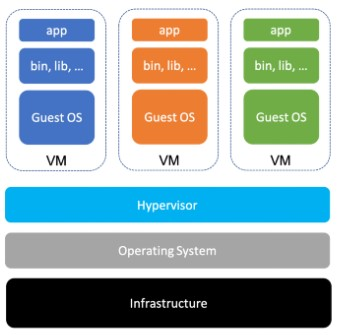
\includegraphics[scale=0.8]{przyklad1.jpg}
}


%Główne problemy wirtualizacji
\frame{
	\frametitle{Główne problemy wirtualizacji:}
	\centering
	\begin{itemize}
		\item Każda wirtualna maszyna potrzebuje własnego systemu operacyjnego.
		\item System operacyjny zajmuje pamięć wydzieloną dla konkretnej wirtualnej maszyny.
		\item Systemy operacyjne mogą się powtarzać - redundancja.
		\item Ewentualne koszty licencji w przypadku własnościowych systemów operacyjnych.
	\end{itemize}
}


%Kontenery
\section{Kontenery}
\frame{
	\frametitle{Kontenery}
	\centering
	
	Metoda spakowania aplikacji wraz z niezbędnymi bibliotekami, plikami i najważniejszymi dla jej działania funkcjami systemu operacyjnego.\\
	\vspace{1em}
}


\frame{
	\frametitle{Najczęściej używane platformy do pracy z kontenerami}
	\centering
	
	
\includegraphics[scale=0.4]{docker.png}
	
\includegraphics[scale=0.8]{openshift.jpg}
}


%Działanie kontenerów
\section{Działanie kontenerów}
\frame{
	\frametitle{Działanie kontenerów}
	\centering
	
	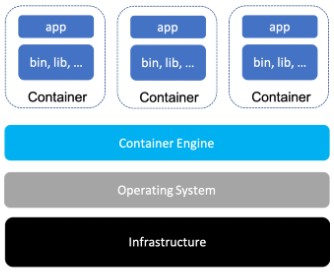
\includegraphics[scale=0.8]{przyklad2.jpg}
}

\frame{
	\centering

	Uruchomione kontenery działają niezależnie od siebie, są bardzo lekkie i nie wymagają tak dużej ilości zasobów w porównaniu do wirtualizacji.\\
	\vspace{1em}
	Proces ich uruchamiania i niszczenia jest bardzo szybki.\\
	Cykl życia kontenera oparty jest na zasadzie, że w razie problemów zawsze można go odtworzyć. 
}


\section{Zalety konteneryzacji}
\frame{
	\frametitle{Główne zalety kontenerów:}
	\centering
	\begin{itemize}
		\item Przenośność aplikacji, brak sytuacji "na moim komputerze nie działa".
		\item Lekkość, więcej pamięci i zasobów do rozdystrybuowania.
		\item Szybkość tworzenia nowych instancji.
	\end{itemize}
}


\section{Różnice}
\frame{
	\frametitle{Różnice}
	\centering
	\begin{itemize}
		\item Wirtualne maszyny uruchamiają się dłużej niż kontenery i wymagają większych zasobów.
		\item Aplikacje graficzne lepiej współpracują z wirtualnymi maszynami, natomiast kontenery lepiej sprawdzą się w architekturze mikroserwisów. 
		\item Zapisane w kontenerze dane nie są trwałe i ulegną zniszczeniu wraz z kontenerem - potrzebna jest dodatkowa rozbudowana konfiguracja w celu ich przechowania.
		\item Wirtualne maszyny lepiej sprawdzą się przy zadaniach wymagających więcej czasu. Cykl życia kontenerów jest krótki.
	\end{itemize}
}


%PODSUMOWANIE
\section{Podsumowanie}
\frame{
	\frametitle{Podsumowanie}
	\centering

	Wykorzystując zarówno wirtualizację i konteneryzację można osiągnąć najlepsze efekty w zarządzaniu infrastrukturą.\\
	\vspace{1em}
	Każde podejście ma swoje wady, lecz dobierając odpowiednie narzędzie do zadania możemy osiągnąć najbardziej optymalne wyniki.
	
}

\frame{
	\frametitle{Bibliografia}

	Docker documentation, https://docs.docker.com (dostęp maj 2022)\\
	\vspace{1em}
	D. Merkel. Docker: Lightweight Linux Containers for Consistent Development and Deployment. Linux Journal, 2014(239):2, 2014.\\
	\vspace{1em}
	M. Uddin. Virtualization for Machine Learning, https://towardsdatascience.com/virtualization-for-machine-learning-da11b7a59070 (dostęp maj 2022).\\

}

\end{document}